\documentclass{article}

\usepackage{xspace}
\usepackage{xcolor}
\usepackage{amsmath}
\usepackage{amssymb}
\usepackage{amsthm}
\usepackage{amsmath}
\usepackage{graphicx}

\newtheorem{conjecture}{Conjecture}[section]
\newtheorem{corollary}{Corollary}
\newtheorem{definition}{Definition}[section]
\newtheorem{example}{Example}

\newcommand{\LTLglobally}{\Box}
\newcommand{\LTLeventually}{\Diamond}
\newcommand{\LTLnext}{\bigcirc}
\newcommand{\Name}{\textit{FormA}\xspace}

\title{COMS 6863 Final Project Status Report: \Name{}}
\author{Max Levatich \& Wonhyuk (Harry) Choi}
\date{\today}

\begin{document}
\maketitle

\section{Introduction}

    Our aim is to design, program, and verify via model-checking a lightweight
	video game called \Name, \emph{Formal verified Asteroids}.
	\Name is based loosely on the classic arcade
    game \textit{Asteroids} \cite{asteroids}; the player controls a small
    spaceship, viewed from a top-down perspective, and must avoid or shoot down
    incoming asteroids from all directions. The player receives points based on
    how many asteroids they destroy and how long they survive.

    \Name{} will be implemented in C, with the help of the low-level rendering
    library SDL. We will use CBMC \cite{clarke2004tool} to model-check
    certain properties of the game as we develop it, including collision
    detection, collision resolution, and input correspondence. We will submit:

    \begin{enumerate}
        \item{The game's code and assets}
        \item{Build instructions, including how to invoke CBMC}
        \item{A correctness specification of the properties checked}
        \item{A final project report detailing our process}
    \end{enumerate}

\section{Game Overview}

    \subsection{Implementation}

        \Name{} is written in C (C11 standard) and depends on Simple DirectMedia
        Layer 2.0 (SDL). SDL is a development library written in C which
        provides a simple low-level interface to the keyboard, audio, and
        graphics hardware necessary to program a video game. We will use CBMC
        to model-check the game (see Section 4).

        We will use the traditional game programming technique of a \textit{game
        loop} located in the main file, where each iteration of the loop
        represents one \textit{frame}, in which we read user input, update the
        game state, and render the game state to the screen. Modules and
        functions will be designed specifically to provide a minimal interface
        to the model-checked portions of our code. We aim to have verified
        modules which encapsulate specific features of the game (e.g. collision
        detection, keyboard input).

    \subsection{Gameplay}

        In \Name{}, the player will use the arrow keys on the keyboard to
        control a ``spaceship''. The up arrow applies a force to the ship in the
        direction that it is facing, while the left and right arrows turn the
        ship in place. This allows the player to navigate a 2D plane which wraps
        around. Asteroids will spawn randomly outside of the boundaries of the
        space with fixed velocities and the player must avoid them or shoot them
        using the spacebar, which will fire a bullet in the direction the ship
        is facing. Staying alive and shooting down asteroids increases the
        player's score. Contact with an asteroid results in a game-over.

        We are entertaining extensions to this core game which provide more
        interesting properties for us to model check, including:

        \begin{enumerate}
            \item{Non-game-ending collisions with ``bouncy'' objects. This allows
                  us to model-check properties like conservation of momentum
                  (subject to energy dissipation).}
            \item{Obstacle courses constructed out of ``planetary'' objects which
                  induce a gravitational field on the ship and asteroids. This
                  allows us to model check the proper application of the force
                  of gravity.}
			\item{``Lives'' and an ``invincibility'' mode after losing a life}
        \end{enumerate}

    \subsection{Algorithms}

        Many of the game's central mechanics revolve around collision detection
        and resolution.

        For collision detection, we will use an Axis-Aligned Bounding Box (AABB)
        algorithm with fine-grained boxes. To enable fine-grained boxes, we may
        also explore classical collision detection optimizations, which prune
        the $n^2$ space of all potential collisions (one for each pair of
        objects) into a set of \textit{candidate} collisions for objects which
        are efficiently determined to be reasonably close
        \cite{moore1988collision, palmer1995collision}. Should we implement any
        optimizations, we will aim to use model checking to show that the
        optimizations are correct; that is, they do not prune any collisions
        which should have happened on a particular frame.

\section{Correctness Specification}

    Our specification will change and grow as we develop the game and discover
    what kinds of properties we can effectively check. Here are some initial CTL
    formulas we plan to check.

    \subsection{Collision Handling}

        $AG(\forall obj. obj \neq ship \implies \lnot touching(obj,ship))$

    \subsection{Input Correspondance}

        $AG(keydown(UP) \implies ship.fx = -sin(ship.theta) * ACCEL\_NORM
                        \land ship.fy = cos(ship.theta) * ACCEL\_NORM)$

        $AG(keydown(LEFT) \land \lnot keydown(RIGHT) \implies ship.omega = ANGULAR\_VEL)$

        $AG(keydown(RIGHT) \land \lnot keydown(LEFT) \implies ship.omega = -ANGULAR\_VEL)$

        $AG(keydown(LEFT) \land keydown(RIGHT) \implies ship.omega = 0)$
	
	\subsection{Asteroid Leaves Screen}
	
		\begin{align*}
			AG((asteroid.x < 0 \lor end < asteroid.x) \land 
			(asteroid.y < 0 \lor end < asteroid.y))
		\end{align*}

\section{Verification Approach}

    To verify our correctness specification (Section 3), we will use the C
    Bounded Model Checker (CBMC). CBMC is capable of statically checking the
    validity of assertions in a C program by unrolling paths through the
    program.

    We plan to express the propositional logic formulas in our correctness
    specification as assertions, preconditions, and postconditions, such that
    CBMC can check them. These assertions will be invoked on every iteration of
    the \textit{game loop}, such that from a zoomed-out perspective where each
    frame of the game is a state transition, they can be viewed as AG() CTL
    formulas.

	We plan to integrate CBMC as a developmental procedure, just like regression testing might be used in a software development cycle.
	Creating the assertions themselves will help with the design process, and model checking will show that we have the correct implementation with respect to the specification.

\section{Project Progress}
So far, we have created the basics of our game, as shown in Figure~\ref{fig:gameplay}.
The game involves a plane and asteroids that move around according to the laws of physics (i.e. velocity and acceleration).

\begin{figure}[!h]
    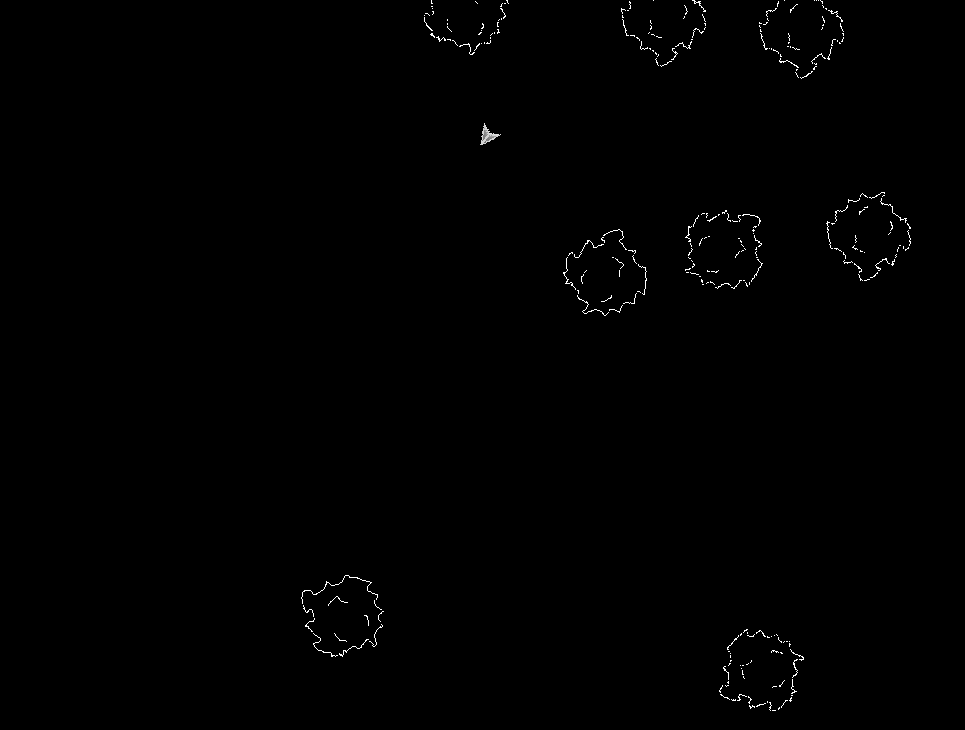
\includegraphics[width=\linewidth]{gameplay.png}
    \caption{Screenshot of \Name}
    \label{fig:gameplay}
\end{figure}

However, we are currently struggling with applying \texttt{CBMC} to our project.
Our game relies on the use of the \texttt{SDL} library, but the library does not work well with \texttt{CBMC}.
A simple file \texttt{main.c} such as 
\begin{verbatim}
#include<SDL2/SDL.h>
int main(){}
\end{verbatim}
results in the following error in Figure~\ref{fig:cbmc-sdl}, even though the code runs properly.
This behavior is consistent whether we use \texttt{cbmc} or \texttt{goto-cc}, and whether we use the \texttt{--no-library} option.

\begin{figure}[!h]
    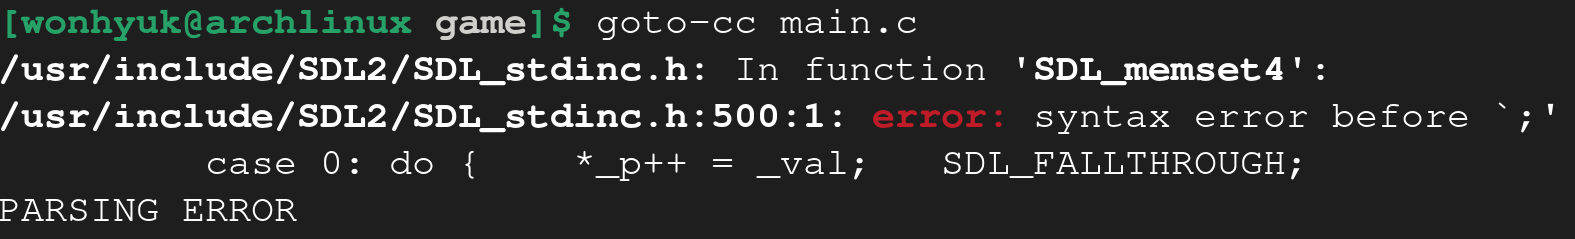
\includegraphics[width=\linewidth]{cbmc-sdl.png}
    \caption{Error with SDL2 and CBMC}
    \label{fig:cbmc-sdl}
\end{figure}

Our current idea is to decouple our codebase from SDL, so that we can check it without SDL, pending any advice or suggestions from the instructors.

\bibliographystyle{IEEEtran}
\bibliography{proposal}

\end{document}
